\documentclass[titlepage]{article}
\usepackage[left=15mm,right=15mm,top=1in,bottom=1in]{geometry}
\usepackage{graphicx}
\graphicspath{ {C:\Users\Nick\Documents\GitHub\3A04\3AO4\doc\intermediateFiles} }

\title{Stone Identification App \\
	Software Requirements Specification}
\author{Genevieve Okon (okong), Sydney Lieng(liengsn),\\
	Niko Savas(savasn), Nick Lago(lagond),\\
	Eric Le Fort(leforte)}
\date{\today}

\begin{document}
\begin{titlepage}
\maketitle
\end{titlepage}
\tableofcontents
\newpage
\section{Introduction}
\label{sec:introduction}
% Begin Section
\subsection{Purpose}
The following Software Requirements Specification (SRS) document will provide an overview of the behaviour of the Stone Identification App that will be developed. This document will include a full description of the application and will outline the functional and non-functional requirements that the system needs to fulfill. To gain a thorough understanding of this application, this SRS is geared towards those who are interested in developing and funding this application. It will give them insight to what the software will do and how it will be expected to perform.
\subsection{Scope}
The Stone Identification App will assist users with the classification of rocks. The system will be able to take in descriptions, such as colour, texture, and size, to recognize the type of rock. When searching through the database, the application will display images of the possible matches, a description, and how much it will cost per gram. In addition, the application will access Google maps API to help narrow the search by location, as well as show others in the area who have also have found similar rocks. Users will also be able to search for rock names and see a description, value and images of the selected rock. The goals of this application is to allow those who are interested in rocks to have a quick access to a database and search through its resources. This application is also used to encourage those who do not know much about rocks to learn more about their qualities. 
\subsection{Definitions, Acronyms \& Abbreviations}
\textbf{Software Requirements Specification (SRS):} a complete description of the behaviour of a system to be developed. It includes a set of use cases that describe interaction betweeen the system and the user/environment.\\
\textbf{Layman's Terms:} describe a complex or technical issue using words and terms that the average individual (someone without professional training in the subject area) can understand, so that they may comprehend the issue to some degree.\\
\textbf{Crash:} when a software stops functioning properly\\
\textbf{Read-only:} cannot write or change the file's contents
\subsection{References}
\textbf{Andrew LeClair.}\\
SE 3A04: Requirements Templates\\
\textit{Department of Computing and Software, McMaster University, January 27/28, 2016}
\subsection{Overview}
The remaining SRS document will include the overall description, functional requirements, and non-functional requirements. It will provide a description of the general factors that affect the product and its requirements in the Overall Description section. The Functional Requirements section will contain all the software requirements to a level of detail. The last section, Non-Functional Requirements, will outline the how the system is supposed to be, such as the look and feel, usability and humanity, performance, etc. 

%%%

% Begin SubSection


\section{Overall Description}
The following section will outline the factors that affect our product and its requirements.\\

\subsection{Product Perspective}
The stone identification app will provide similar functions to rock identification sites, presented in an app to be more accessible and portable. The application will also implement some extra features such as value approximation and marketplaces. The application will work by asking multiple questions to refine the list of rocks suggested by the application. The product will make use of google maps and therefore will not be completely self contained. 
There is no larger system that will be interacting with our application.\\

\subsubsection{Product Functions}
\begin{itemize}

\item If the user finds a rock, the application will display a list of all possible rocks for a match \\
\item Each rock possibility is accompanied by a picture, a description and an approximate value\\
\item The application will display a set of questions as a form that the user can answer to refine the selection of possible rocks\\
\item Once a match has been found, the customer has the option to save rock information to their \"rocks found\" list.\\
\item Customers will be able to remove rocks from their collection\\



\end{itemize}

\subsubsection{User Characteristics}

User restrictions may include:\\
\begin{itemize}

\item No educational restrictions during the identification process, as the use of pictures make this very intuitive\\
\item Some descriptions, and questions about rocks may require a slight knowledge of geology \\
\item Previous experience with phone applications is an asset when using this product\\
\item No technical expertise needed, however users may take some time at first to learn all the features\\

\end{itemize}


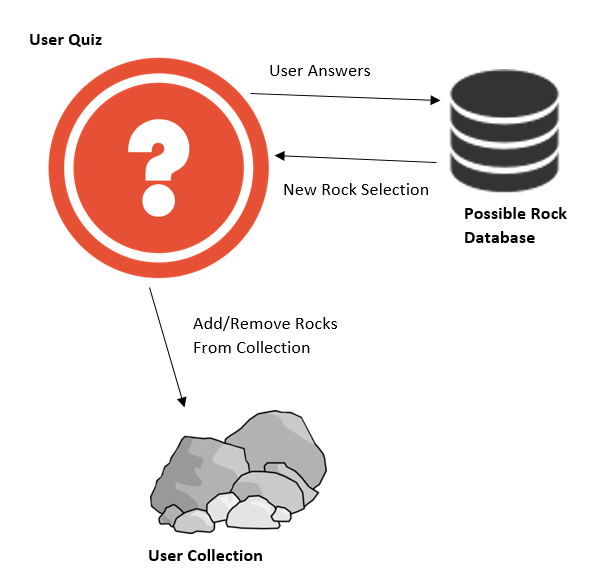
\includegraphics{../resources/Interaction.png}

\subsubsection{Constraints}

\begin{itemize}
\item Possible matches are limited to database space\\
\end{itemize}


\subsubsection{Assumptions and Dependencies}

\begin{itemize}
\item Users have enough space on mobile device to hold the app\\
\item User has enabled GPS function in phone\\
\item Device with application is an android phone\\
\end{itemize}


\subsubsection{Apportioning of Requirements}

Some requirements that may be delayed until future versions:

\begin{itemize}
\item Interacting with other users rock collections, such as viewing, and requesting to purchase \\
\item Messaging system between collectors \\
\end{itemize}
\section{Functional Requirements}
\label{sec:functional_requirements}
\subsection {Business Event: User wants to identify a rock}
	\subsubsection {Viewpoint: Everyday User}
		\begin{itemize}
			\item The application will allow the user to input information about texture, colour, and/or size of a rock.
			\item The application will estimate the type of rock based on user-inputted texture, colour, and/or size.
			\item The application will suggest rocks based on the user's location.
		\end{itemize}
	\subsubsection {Viewpoint: Developer}
	\subsubsection {Viewpoint: Security Expert}
\subsection {Business Event: User wants to update the database}
	\subsubsection {Viewpoint: Everyday User}
		\begin{itemize}
			\item The every day user will not be able to modify the database.
		\end{itemize}
	\subsubsection {Viewpoint: Developer}
		\begin{itemize}
			\item The developer will be able to update the database with new information
		\end{itemize}
	\subsubsection {Viewpoint: Security Expert}
		\begin{itemize}
			\item The security expert must be able to manage developer access to the database
		\end{itemize}
\subsection {Business Event: User wants to save a rock they've found}
	\subsubsection {Viewpoint: Everyday User}
		\begin{itemize}
			\item The user will be able to add a rock from their matched list to a ``Found Rocks" list.
		\end{itemize}
	\subsubsection {Viewpoint: Developer}
		\begin{itemize}
			\item The developer will not be able to access an individual user's found rock list.
		\end{itemize}
	\subsubsection {Viewpoint: Security Expert}
		\begin{itemize}
			\item The security expert shall ensure that only the user can see their own rock list.
		\end{itemize}
\subsection{Business Event: Application identifies cost per weight }
\subsubsection{Viewpoint: Application}
\begin{itemize}

  \item The application shall show the cost of the rock according to the weight of the rock. 
  \item The application shall show the cost per gram of the rock.
  \end{itemize}
  \subsubsection{Viewpoint: Everyday User}
  \begin{itemize}
  \item The user shall be able to enter the weight of the rock found in the application.
  \item The users shall be provided with possible places to sell rocks found.
  
\end{itemize}

\subsection{Business Event: Application displays image}
\subsubsection{Viewpoint: Application}
\begin{itemize}
\item The application shall display images of possible matches for rocks according to user input.
\end{itemize}
  \subsubsection{Viewpoint: Everyday User}
  \begin{itemize}
  \item The user shall be able to view the image of the final rock match found.
\end{itemize}


\subsection{Business Event: User searches for rock name}
\subsubsection{Viewpoint: Application}
\begin{itemize}

  \item The application shall search for the name of the rock according to the categories the user chooses.
  \item The application shall eliminate rocks that do not match the criteria as the user specifies more about the rock found. 
  \item The application shall be able to access the database to find information about the possible rock. 
  \end{itemize}
    \subsubsection{Viewpoint: Everyday User}
  \begin{itemize}
  \item The user shall be able to view name, location and properties of rock match found. 
\end{itemize}


\section{Non-Functional Requirements}

The following section will outline the various non-functional requirements that pertain to the Rock Identification app.

\subsection{Look \& Feel Requirements}
These requirements dictate how the final product will appear to the user. The overall goal will be to make the app's look \& feel in a way that promotes simple and efficient use by the average user.
\subsubsection{Appearance Requirements}
\textbf{Ap1:} The program shall use appealing colour schemes determined by the designers.\\

\noindent\textbf{Ap2:} The program's appearance shall be designed in a way that it does not distract from usage of the system.\\

\noindent\textbf{Ap3:} The program shall be easy to see even in environments with high background light (i.e. outdoors).

\subsubsection{Style Requirements}
\textbf{S1:} The program shall uphold a simple design with each page displaying only the necessary information.

\subsection{Usability \& Humanity Requirements}
\subsubsection{Ease of Use Requirements}
\textbf{EOF1:} The program shall be usable by any user between the ages of 8 and 90 with basic knowledge of how apps function.
\subsubsection{Personalization \& Internalization Requirements}
\textbf{PI1:} The program shall keep a record of all rocks discovered by the user.
\subsubsection{Learning Requirements}
\textbf{Le1:} The user shall need to know what the basic qualifying characteristics of rocks mean and how to check for them.
\subsubsection{Understandability \& Politeness Requirements}
\textbf{UP1:} The program shall be able to be used by any people as defined in the requirement EOF1 without any prior training
\subsubsection{Accessibility Requirements}
\textbf{Ac1:} The program shall utilize the largest text possible while maintaining it's aesthetic appeal.\\

\noindent\textbf{Ac2:} The program shall include information in \textit{Layman's Terms} to support the more technical information.

\subsection{Performance Requirements}
\subsubsection{Speed \& Latency Requirements}
\textbf{SL1:} Time computing possible matches and displaying those results shall never exceed 1 second.\\

\noindent\textbf{SL2:} Time to start the program shall never exceed 3 seconds.
\subsubsection{Safety Critical Requirements}
N/A
\subsubsection{Precision \& Accuracy Requirements}
\textbf{PA1:} The program shall display the correct rock that matches the descriptors (assuming they are correct) 95\% of the time.\\

\noindent\textbf{PA2:} The program shall display the correct rock that matches the descriptors (assuming small mistakes by user being possible) 80\% of the time.
\subsubsection{Reliability and Availability Requirements}
\textbf{RA1:} This system is available on the user's machine and does not rely on other factors to function. This program should be available 100\% of the time.\\

\noindent\textbf{RA2:} The program shall \textit{crash} no more than once per hour of accumulated runtime.
\subsubsection{Robustness or Fault-Tolerance Requirements}
\textbf{RFT1:} The program shall be designed in a way that faulty inputs are not possible to select.
\subsubsection{Capacity Requirements}
\textbf{CR1:} The program is designed to work independently on a single piece of hardware. If the program operates as stated in the other requirements on one device, this requirement will be satisfied.
\subsubsection{Scalability or Extensibility Requirements}
\textbf{SE1:} The program shall store only the past 100 rocks found by the user.\\

\noindent\textbf{SE2:} The program shall be designed in a way that adding new rocks to the database is possible after deployment without major changes.
\subsubsection{Longevity Requirements}
\textbf{Lo1:} The product shall be designed in a modular way so as to allow future anticipated change.

\subsection{Operational \& Environmental Requirements}
\subsubsection{Expected Physical Environment}
\textbf{EP1:} The program will primarily be operated outdoors. The program shall be designed such that non-extreme environments will not affect usability or performance.
\subsubsection{Requirements for Interfacing with Adjacent Systems}
\textbf{RIA1:} The program shall interface with Android Jelly Bean (4.1.x) and higher.
\subsubsection{Productization Requirements}
\textbf{Pro1:} The program shall come packaged with all required libraries necessary to readily interface with Android Jelly Bean (4.1.x) and higher.
\subsubsection{Release Requirements}
\textbf{R1:} The program shall be ready for release of version 1.0 by April $3^{rd}$, 2016.

\subsection{Maintainability \& Support Requirements}
\subsubsection{Maintenance Requirements}
\textbf{MS1:} The product shall store its data in such a way that it will only require deleting the last lines of the data file to restore to a previous state as necessary.
\subsubsection{Supportability Requirements}
\textbf{Su1:} The program shall follow a modular design pattern. No more than 10\% of modules will be so rigid they can only operate in the exact implementation of the current system.
\subsubsection{Adaptability Requirements}
\textbf{Ad1:} The program shall be able to integrate new types of rocks into its identification system without affecting any other component's operation.

\subsection{Security Requirements}
\subsubsection{Access Requirements}
\textbf{AR1:} Accessing the identification feature will not require credentials, however, accessing the previous rocks discovered or adding new rocks will require the user entering their password.
\subsubsection{Integrity Requirements}
\textbf{In1:} The rock data stored locally will be encrypted and compared against fixed values as needed to verify there has not been any tampering.\\

\noindent\textbf{In2:} The user's password will be padded and stored encrypted with two different methods of encoding. Both methods of encoding must return the same password to ensure there has not been any tampering.
\subsubsection{Privacy Requirements}
\textbf{Pri1:} The program will not disclose any information about the user to third-parties without permission.
\subsubsection{Audit Requirements}
N/A
\subsubsection{Immunity Requirements}
\textbf{Im1:} The program shall make all files that do not change due to normal program operation \textit{read-only} in the file system.\\

\noindent\textbf{Im2:} The program shall make an announcement to the user if any files hold unexpected data.

\subsection{Cultural \& Political Requirements}
\subsubsection{Cultural Requirements}
\textbf{Cu1:} This program shall not include any symbols, statements or anything of that nature that may be found offensive to anyone's culture.
\subsubsection{Political Requirements}
\textbf{Po2:} This program shall not include any symbols, statements or anything of that nature that display any sort of political stance.

\subsection{Legal Requirements}
\subsubsection{Compliance Requirements}
\textbf{C1:} The program shall not retain sensitive data about the user without the user's permission.
\subsubsection{Standards Requirements}
N/A


\appendix
\newpage
\section{Division of Labour}
\label{sec:division_of_labour}
% Begin Section
\begin{center}
\begin{tabular}{ | p{6cm} | p{6cm}| p{4cm} | } 
\hline
Name& Contribution & Signature\\ 
\hline
Genevieve Okon & Functional Requirements & \\ 
\hline
Eric Le Fort& Non-Functional Requirements&  \\ 
\hline
Nick Lago& Overall Description  &   \\ 
\hline
Niko Savas& Functional Requirements&   \\ 
\hline
Sydney Lieng& Introduction&   \\ 
\hline
\end{tabular}
\end{center}
% End Section

\end{document}
%------------------------------------------------------------------------------